\chapter{Design}

\section{Application Structure}

\subsection{Progressive Web Applications}
The Bazo Wallet application is designed as a Progressive Web Application.
\subsection{Network Communication}
\subsection{Interfaces}

\section{Transaction Information} \label{transactioninfo}
One requirement, that is that Bazo coins can be exchanged between users without direct involvement or administration from the service provider was incorporated into the core design of the Bazo currency. To fulfill said requirement it is vital that transaction informations can be shared between users of the Bazo Wallet. This section outlines how transaction information can be shared with the Bazo Wallet.
%Search for papers, resources etc.
Sharing transaction information in native applications is often achieved with technologies such as NFC, Bluetooth or by encoding and reading transaction information from a Quick-Response Code.
\subsection{Schema}
In order to communicate Bazo Transactions to other devices and applications, an URI Scheme was designed to hold transaction information, so that a requesting party can communicate it. The grammar and structure for the schema followed the \cite{bip21} 21st Bitcoin Improvement Proposal for an URI scheme since it contained all necessary elements to fulfill the requirement. The URI Schema consists of a required part which holds the protocol name and the recipient's fully qualified bazo address.


\[
\underbrace{\overbrace{bazo:}^{\mathrm{protocol}}\overbrace{MIGfMA0GCSqGSIb3DQEBAQUAA4GNADC}^{\mathrm{bazo address}}}_{\mathrm{required components}}
\underbrace{\overbrace{?amount=123}^{\mathrm{amoun t}}\overbrace{?label=1 Coffee}^{\mathrm{label}}\overbrace{?message=Message}^{\mathrm{message}}}_{\mathrm{optional components}}
\]


% reference nfc bridge
This implies, that the Bazo Wallet and other applications that need to interact with it need to be able to encode and decode transaction information as supplied in the described grammar.
For the web-based wallet this transaction info should also be an optional parameter of the URL of the payment page. This allows that a complete URI to the payment page with all required transaction information can be shared among users or between merchants and users.
This enables to encode complete transaction information as well as a an URI to the application page with the transaction information into media such as a QR-Code. This has the benefit, that all users of the Wallet can exchange payment information without having to know about the Schema.
Since merchants frequently have more advanced payment systems and don't want to encode payment information into media such as QR-Codes for each new transaction, the payment page of the Wallet also needs to be able to accept additional parameters, by which the Wallet can then query the transaction amount from a service.
The schema below shows the URI endpoint of the payment page, together with additional parameters that can be supplied to have the payment page prefilled with transaction information. This procedure is further described in Figure\ref{fig:POS}.
\[
\underbrace{\overbrace{https://host/:}^{\mathrm{Host}}\overbrace{/auth/user/send}^{\mathrm{payment page}}}_{\mathrm{required components}}
\underbrace{\overbrace{posid=323}^{\mathrm{POS identification}}\overbrace{?paymentinfo=bazo://123123}^{\mathrm{transaction info}}}_{\mathrm{optional components}}
\]

The implementation of the module to encode and decode bazo encoded transaction information is described in \ref{xy}.
%reference impl

\subsection{Device Sharing}
In order to explore further possibilities on how to extend the browser support for native API's a Proof of Concept was implemented. The PoC was targeted to the android Platform, since NFC support is still fairly limited on iOS devices at the time of the design. The PoC, further referenced as 'NFC Bridge', should run as a background service and enable two processes.
\begin{enumerate}
\item Reading NFC devices:
The application should be registered as a handler for NFC messages. If an NFC message is read from another NFC device such as another active device or an NFC Tag, the user is prompted with applications that can handle the data format. If the user selects the NFC Bridge application, the data received from the NFC Adapter should be parsed and the user prompted with the Payment page of the Bazo Wallet. The payment page is then prefilled with the payment information extracted from the NDEF message.
\item Pushing to NFC devices: The NFC Bridge application should allow the PWA-based Bazo Wallet to push handover encoded transaction information which can then be pushed to NFC devices and tags.
The first design sketch included that communication between the Bridge application and the Bazo Wallet is done through an HTTP or Websocket. This implied that the NFC Bridge is running as a background service, listening for NFC messages and keeping the server alive.
Since the android platform allows starting the application when an NFC message is received through the configuration of application intents, this design was preferred.
\end{enumerate}

\subsection{Merchant options}\label{fig:tps}
In order to completely support the payment process, which does require interaction of the application with backend services from the financial service provider, interfaces need to be integrated into the application.
This is also necessary since some platform do not support WebNFC in the browser, which means that the payment process can not be carried out in a complete device-to-device manner. On iOS devices support for NFC access is restricted to native API's and the functionality is limited to reading passive NFC Tags.
In order to get the complete payment process depicted, the payment process that is to be developed can be described as follows. The user of an iOS device can use his any NFC Tag Reader app from the app store. Before the payment process can be started, the merchant needs to supply payment information in form of a correct bazo address as well as some token that represents the Point-of-sale system. The merchant should have the possibility to write these informations to the NFC Tag at the POS, using the Mobile Wallet application.
Once this set up is in place, the user will approach the POS System and may start the payment process. The cashier will scan the items, and the POS System will automatically associate the POS ID with the transaction amount. The user can now use any existing iOS or android application to read the NFC tag. Since both payment and transaction information is encoded in a URL, the user is taken to the payment page of the Mobile Wallet, where the POS ID is used to query the transaction amount from the POS System. Since the Bazo Address is supplied in the URL as well, the user can confirm the payment. Once confirmed the Mobile Wallet will sign the transaction and send it into the Bazo network. Figure
\ref{fig:POS} shows the process of transferring transaction information and transaction issueing under the constraint that a third party service needs to be queried.

\begin{figure}
\centering
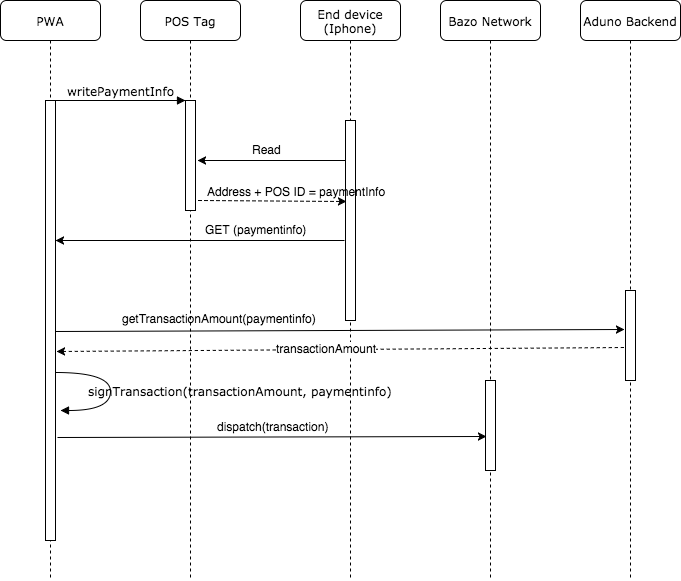
\includegraphics[width=1\textwidth]{diagrams/POS_flow.png}
\caption{\label{fig:POS}Transferring payment information across devices using NFC.}
\end{figure}

\section{Communication}
%% Interfaces includes integration of existing services
\subsection{Bazo Interfaces}
\subsection{Payment System Interfaces}

\subsection{Security Considerations}







\chapter{Implementation}
\section{Architecture}
\subsection{User Interface}
\subsection{Storage}
\subsection{State}
\subsection{Network Handling and Communication}

\section{Transaction Sharing}
Requesting payments is a core requirement for the Bazo Wallet to qualify as a payment system for end-users. The design of the sharing process and the data model were explained in \ref{transactioninfo} This section explains how sharing transaction data across devices was implemented.
\subsection{Web APIs and Browser Support}\label{browsersupport}
At the time of writing, more and more native API's are made available for the Web.
The API specification for NFC connectivity is still in draft \cite{webnfc}. However, partial implementations of the API are available in Google Chrome on android devices. Other user-agents and platforms do not yet support the feature although some have expressed intent to implement. The implementation state in Google Chrome is not documented thoroughly, so the specifications guidelines and Google Chrome's source code was the only way to obtain information on the subject apart from testing.
% TODO Reference state for Webkit, moz, IE.
For the prototype, the feature was implemented for Google Chrome on android.
In order to allow web-nfc in Google Chrome, there need to be two flags set to enable the experimental implementation.
"Experimental Web Platform features" and "webnfc". The first of these flags will show the nfc object in the navigator object of the browser. However, this does not mean that the hardware does support web-nfc. The latter flag can only be set on devices whose hardware actually supports NFC.
After extensive testing, it became clear that the current implementation of Google Chrome only allows devices to use NFC functionalities such as reading and writing to them with NFC tags. Performing these actions to active NFC devices such as a smartphone will throw the corresponding error according to the specification draft \cite{webnfc}.

Another challenge posed the creation and signing of Bazo transactions in the browser. Since not all data-types that are usually available in C-like structs are available in the browser, and browser support is still not widely adapted, a bridging solution had to be implemented.
The structure of a Funds Transaction can be seen in figure \ref{fig:FundsTX}

\begin{figure}
\centering
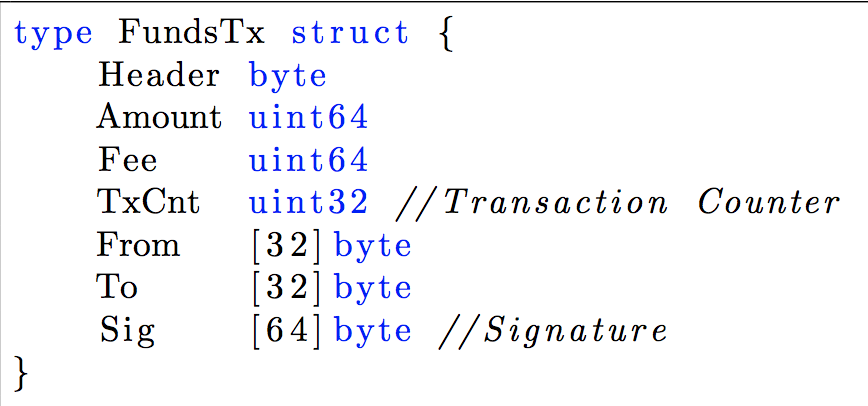
\includegraphics[width=1\textwidth]{diagrams/AccountTx_struct.png}
\caption{\label{fig:FundsTX}Structure of a FundsTx in Bazo.}
\end{figure}.


\subsection{NFC}
\subsection{NFC Bridge}\label{nfcbridge}
Due to limited browser support for Native API's such as webNFC, see \ref{browsersupport}, a prototype was discussed and implemented in this thesis. The prototype involved a native android application that should enable the web application to forward transaction information that could be forwarded to NFC capable devices using the Android Beam technology.
The design and requirements of such an application was outlined in \ref{xy} and the two main functional requirements for the application were presented.
Reading NFC messages from passive and active devices, was achieved without implementing it in the android application. This was done by changing the data model for transaction information to one that can be expressed in a single URL. With this media type, it is possible to use the tag dispatching system in android. This would work as follows:
1. An NDEF message is received when the android device is unlocked and NFC enabled.
2. The NDEF message for this application contains just one URL. Through android's intent system the application that fits best is started.
3. If the Bazo Wallet PWA was previously installed on the android device, an intent filter is present for the origin URI of the PWA. This will result in the PWA being opened with all transaction data passed as parameter.
4. If the Bazo Wallet PWA is not installed there will be no intent filter requesting the data. The user is then prompted with all applications that can handle an URI, such as a Web browser. If a browser is selected, then the Bazo payment page is opened with all transaction data passed as a parameter.
%https://developer.android.com/guide/topics/connectivity/nfc/nfc.html

Writing the transaction data to other android devices was implemented using the Android Beam technology.
The transaction data can be passed to the NFC Bridge by either manually entering it into a form or by passing it as data through an intent. Passing data to the application through parameters has the benefit that web applications can generate links that will take the user to the application. Such a link can contain further data, which would be set to the transaction data the user wants to share with another android device.
If the android phone is held against another Android Beam enabled device, the NFC Bridge application will automatically set the appropriate transaction data encoded as an NDEF message and push it to the other device.

At the time of writing, NFC support for iOS platforms was just released for their most recent publicyl available version, iOS 11. The NFC functionality offered to iOS developers covered writing and reading to NFC tags on the iPhone 7 and iPhone 7 Plus \cite{corenfc}. Thus, an NFC Bridge application similar to how it was developed for android would not extend the functionality of existing generic NFC applications. The NFC fallback capabilities with the Bazo Wallet on iOS are outlined in chapter \ref{xy}.
\subsection{Bluetooth Low Energy}
\subsection{Quick Response Codes}
\subsection{Fallback Solutions}
Subsections of chapter 4.2 outlined how existing native and web-enabled API's were leveraged for the Bazo Wallet to share transaction data. This section documents the fallback solutions that were evaluated for devices or platforms that lack the support for the API, either natively or on the web.
For android, the complete functionality of NFC could be leveraged. Writing and reading NFC tags was implemented with the web-nfc API. Complete peer to peer communication was enabled by developing an API bridge, see \ref{nfcbridge}.
As iOS platforms only support native API's when communicating over NFC and peer to peer mode is not yet included, the fallback solution to use NFC on iOS devices can be described as follows. Since all transaction data can be encoded into a single valid URL, merchants and users can transfer their transaction data to an NFC tag. This can be done with any generic NFC application or, on an android device, with the Bazo Wallet itself. iOS users can then scan the NFC tag with their preferred generic NFC application. This will open the Payment page of the Bazo Wallet, prefilled with all necessary transaction data.
\subsection{Transaction Encoding}

\section{Blockchain Interaction}\label{blockchaininteraction}
Actual network communication with the Bazo network in a trustless way posed the most difficult technical challenge for the application. The following areas had to be evaluated:

1. Building the transaction data in the schema defined in the Bazo protocol. \ref{fig:AccountTx}.
Due to technical limitations of the browser, this application context is not suitable to fullfill the requirements of a light client implementation. Reasons for this are lack of tcp communcation support, storage and data structures.
To overcome these limitations, native application wrappers for the light client written in Go were evaluated. This approach would have the advantage that each customers doesn't have to maintain a complete copy of the blockchain but transactions can be verified in trustless way. However, the current state of project that enables the mobile bindings for go did not support all networking and data structure needs to fulfill the requirement. \cite{godocs}
2. Signing the transaction data with the appropriate algorithms.
3. Verifying transaction and account information.
In order to run the Bazo Wallet as trustless as possible, the application has to maintain at least a certain amount of the blockchain to verify information. For the Bazo Wallet this would mean that the Bazo Wallet itself needs to verify blocks and transactions, or that the Bazo Wallet needs to talk with a trustworthy Bazo client. The latter approach would have been envisioned as a native application that would run on each mobile device.
The first approach was not suitable, since the lack of support for certain data types and communication protocols are present in the Browser. The latter approach could not be implemented with the given resources. However, native implementations of the Bazo Client for Android and iOS are technically feasible.

% link to gomobile, link to evaluation & future work


\subsection{Bazo Client Web interface} \label{bazoclientwebinterface}
\subsection{Transaction Signing}\label{transactionsigning}
Due to limitations of the browser for C-like structures as they would be required to create a FundsTx \ref{fig:FundsTX}, an interface had to the Bazo client had to be developed. 
The process of obtaining transaction information, requesting a new transaction, signing and dispatching it into the network is shown in figure \ref{fig:TransactionProcess}.
1. The application queries the necessary account information to request a transaction struct in a later step. This is a necessary step, since the TxCount of the transaction has to be correct in order for the transaction to be valid.
2. With the account information, the web application can send a request to the web service to create a new FundsTx struct. The Bazo client creates the appropriate structure, hashes it using the SHA3-256 algorithm and returns it to the Wallet.
3. The Wallet is now in charge of asking the user about its private key, signing the received transaction hash and sending it to the Bazo client.
\begin{figure}
\centering
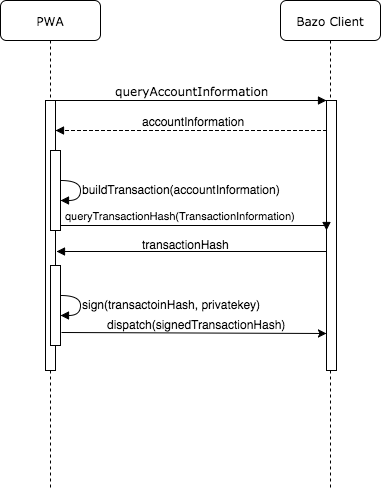
\includegraphics[width=0.75\textwidth]{diagrams/transactionProcess.png}
\caption{\label{fig:TransactionProcess}Structure of a FundsTx in Bazo \cite{lisg}.}
\end{figure}.

This approach is comparable to the mechanism employed in the official JavaScript API of the Ripple currency \cite{ripplelib}.
Figure \ref{ripplesendTx} demonstrates how a transaction can be sent with the Ripple cryptocurrency.
L1: A connection to an interface is opened over a Websocket. 
L3: A request is made to obtain relevant data and instruction for the payment.
L5: The data returned from preparing the transaction is signed.
L7: The API submits the signed Transaction over the WebSocket


\begin{figure}
\centering
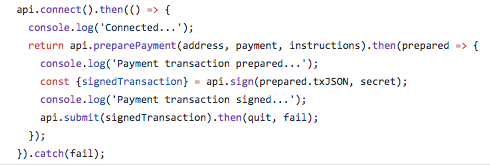
\includegraphics[width=1\textwidth]{diagrams/ripplelibSendTX.png}
\caption{\label{ripplesendTx}Programmatically creating, signing and sending a transaction with Ripple-lib\cite{ripplelib}.}
\end{figure}.


\subsection{Data Queries}
\subsection{Client Integration}
Chapter \ref{bazoclientwebinterface} explained the interaction between the Bazo Wallet and the Bazo light client over a web interface.
This chapter explains contexts in which the bazo client can be run, consequences and documents the efforts of porting the light client to mobile devices.
Due to the security constraints one needs to be consider when interaction with other sources in a PWA, the Bazo client web interface has to be in a secure context. This would mean that an SSL certificate needs to be installed or the server needs to accessible through a secure reverse tunnel.
This makes mobile devices as a runtime unsuitable, since an SSL certificate can not easily be installed for each mobile device. However, a proof of concept was developed to show that mobile devices are technically feasible to run the client. In chapter \ref{blockchaininteraction}, it was explained that binding the bazo client that was written in the go programming language in native android development using the official tools was not possible due to a lack of support for data-types. The following xy explain how the bazo client was ported to the android operating system for ARMv5 devices.
To port the complete bazo client without any modifications to the android operating system the application was compiled  using the clang compiler. The compiler can be obtained through androids official NDK or it can be compiled from scratch. The complete toolchain was compiled targeting the arm architecture, and android API version 21 on a darwin x64bit system. The clang compiler of the toolchain was then used to configure the go environment for cross-compilation. The bazo client could then be compiled for android by configuring the golang environment for arm architectures and to use the freshly compiled clang compiler.
The binary was then copied to an android device an ran in the scope of an existing application. This is a necessary step for binaries that are run on devices were root access is not given. The application performed well, so that ngrok was used to create a secure reverse tunnel. With this in place the web application was able to interact with the bazo client running on the same device but accessible through the secure context.
This Proof of Concept could be leveraged to create an actual android application wrapping the binary. However, a solution to configure SSL appropriately would need to be found.
% reference in future work

\section{Testing}


\chapter{Evaluation}
\section{Prototype Evaluation}
\section{Comparison}
\section{Limitations}
\section{Future Development}
\section{Future Work}
\newpage

\chapter{Summary and Conclusions}
